Many models of physics beyond the Standard Model (SM) predict the
existence of new heavy particles which couple to quarks and/or
gluons. 
Such heavy particles could be produced in proton\text{--}proton
collisions at the Large Hadron Collider (LHC) and then decay into
quarks and gluons, creating two hadronic jets in the detector. 
In the SM, dijet events are produced mainly by quantum chromodynamics
(QCD) processes. 
QCD predicts dijet events with a smoothly decreasing invariant mass
distribution, \mjj. 
A new particle decaying into quarks or gluons could appears instead as
a resonance in the \mjj spectrum.  

A search for new physics in the dijet mass distribution was performed
using $\sqrt{s} = 13$~\TeV\xspace data collected between years 2015 and
2018 \cite{Aad:2019hjw}. 
%with the  95\% CL lower limits on the masses given in Table~\ref{tab:Limits2018}. 
Most of the strategies and methods of the analysis presented here are
mostly unchanged with respect to the previous iterations of the
analysis, which can be reviewed in great detail in the internal note
~\cite{Nishu:2646455}. 

\todo[inline]{To write about updated statistical framework.} 

%For these reasons, searches in dijet events are often amongst of the first searches done when a hadron
%collider reaches a new energy frontier\footnote{See Ref.~\cite{Harris:2011bh} for a review of the history
%of these searches from UA1 and UA2 to the LHC Run 1.}.  Increases in collision centre-of-mass energy, \s , 
%dramatically improves the reach of searches for potential high-mass signals. 
%Increases in the integrated luminosity of the data samples results in much smaller improvements and requires significant 
%improvements in the understanding of systematic uncertainties. 

%The increase in collision center-of-mass energy \s\ from
%8 to 13~\TeV\xspace dramatically enhances parton luminosities at multi-\TeV\xspace energies
%(Fig.~\ref{fig:partonluminosity}) and thus the production rates of potential high-mass signals.

%\begin{table}[htbp]
%  \caption{The lower limits on the masses of benchmark signals at 95\% CL from \cite{Aad:2019hjw}.%}
%  \centering
%  \begin{tabular}{l|c|c|c}
%    \hline\hline
%    \multirow{2}{*}{Category} & \multirow{2}{*}{Model} & \multicolumn{2}{c}{Lower limit on signal %mass at 95\% CL} \\ 
%    & & Observed & Expected \\\hline
%    \multirow{6}{*}{Inclusive} & $q^*$ & 6.7~\TeV\ & 6.4~\TeV\  \\
%    & QBH & 9.4~\TeV\  & 9.4~\TeV\ \\
%    & \Wprime & 4.0~\TeV\ & 4.2~\TeV\  \\
%    & $W^*$   & 3.9~\TeV\ & 4.1~\TeV\ \\
%    & DM mediator \Zprime, $g_\text{q}=0.20$ & 3.8~\TeV\ & 3.8~\TeV\ \\
%    & DM mediator \Zprime, $g_\text{q}=0.50$ & 4.6~\TeV\ & 4.9~\TeV\ \\\hline
%  \end{tabular}
%  \label{tab:Limits2018}
%\end{table}

If the resonant data sample can be divided based on the type of
parton that initiated the jets, the sensitivity of the search for some
rescounaces could be increased. 
The fraction of events as a function of  
the dijet mass from QCD  simulated with a  \textsc{Pythia~8.186}~\cite{pythia8} and the leading-order NNPDF2.3~\cite{Ball:2012cx} 
parton distribution functions (PDFs) is shown in Fig.~\ref{fig:quarkgluonfraction}. 
This suggests that tagging quark and gluon jets should be able to improve the sensitivity of searches for new particles. 
ATLAS has published a study \cite{ATL-PHYS-PUB-2017-009} showing that jets can be tagged as quark or gluon jets 
based on the number of charged particles with transverse momentum (\pt ) above 500\,MeV. 
In this note we present the analysis for the whole combined 2015 and
2016 $\sqrt{s} = 13$~\TeV\xspace dataset using quark 
and gluon tagging  based on charged-particle constituent multiplicity.

\todo[inline]{Update Fig 1 with dijet fractions nicer plot...}
\begin{figure}[htb]
 \centering
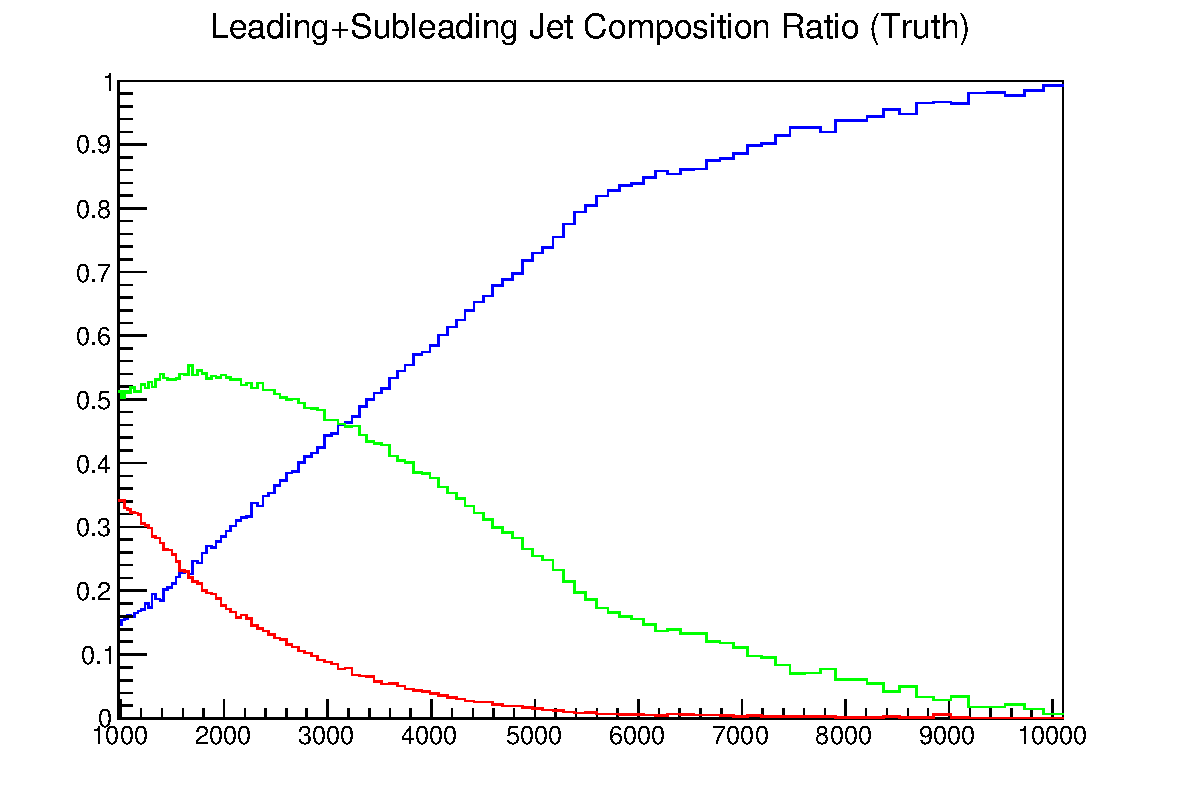
\includegraphics[width=0.75\textwidth]{figures/introduction/truthCompositionRatio.pdf}
\caption{The fraction of dijet events that are initiated by quark-quark events (blue), quark-gluon 
events (green) and gluon-gluon events (red) in simulated data.  \label{fig:quarkgluonfraction}}
\end{figure}

\subsection{Overview of the analysis}
\label{sec:overview}

First, we demonstrate using toy MCs that tagging quark and gluon jets can, in principle, make significant 
improvements to the sensitivity of the resonance search.

The subsequent analysis of the data will follow previously used in the inclusive analysis of the full Run-2 data 
\cite{EXOT-2016-21,Nishu:2646455}. This is reproduced here for convinience. 

We analyze dijet events using the dijet invariant mass \mjj\  (described in Section \ref{sec:observables}).

The initial analysis steps are

\begin{enumerate}
\item Unprescaled single-jet triggers are used to collect events containing
highly energetic jets (Section~\ref{sec:trigger})
\item High-\pT\xspace jets are reconstructed, identified, and calibrated according to recommendations, with techniques
prepared in tandem between the analysis team and the
JetEtMiss group (Section~\ref{sec:jet_reconstruction}).
\item After calibration, bulk processing of the data, and production of a standardized xAOD derivation, events are selected with very similar kinematic 
criteria as in previous dijet searches (Section~\ref{sec:base_selection}). The data and Monte Carlo used are described in
Appendices~\ref{sec:datasample} and ~\ref{sec:qcdsample}. Prior to the availability of the data in the final
analysis, analyzers closely monitor the on-line and offline data preparation and
quality efforts for advance warning of problems.%(Appendix~\ref{app:dqchecks}).
\item When the data are available for inclusion in the analysis, the jet kinematics, calibration performance, 
and quality are monitored at the analysis level (Table~\ref{tab:jetCalibration} in Section~\ref{sec:event_selection}).
\end{enumerate}

Statistical tests are employed in a
\textit{search phase}, will be added to the Section~\ref{sec:statistical_framework}, to determine whether the 
data are compatible with a background expectation. 
A localized excess (i.e. a bump) on the smooth \mjj\  distribution
is the target of the resonance analysis.
The background model is derived from a fit to the \mjj\ distribution.
The background estimation strategy is described in Section~\ref{sec:background_estimation}.
A description of systematic uncertainties will be added to 
Sections~\ref{sec:systematic_uncertainties}. 
%In case either method observes a significant excess, additional tests in the search phase
%are detailed in Section~\ref{sec:cross_checks}. 
%The results of the search phase will be shown in Section~\ref{sec:search_results}.

If no new phenomena is found, a ~\textit{limit setting phase} is used
to constrain a set of signals. 
%\begin{itemize}
% \item Limits on benchmark signals:
%\begin{itemize}
% \item Excited quarks.
% \item Limits on Quan
% \item Limits on hadronically decaying \Wprime .
% \item Limits on hadronically decaying \Wstar .
% \item Limits on dark-matter inspired \Zprime\ models.
The techniques and tools used for the limit setting are described in
Section~\ref{sec:limits}. 
%The systematic uncertainties considered on the benchmark signals are
%detailed in Section~\ref{sec:systematics_signal}.
%Each of the following sections clarifies what is consistent
%with the previous iteration and what has been further developed.

\subsection{Strategy for applying quark-gluon selection to the full Run-2 data.}
\label{sec:2018data}

The analysis strategy, cuts, and other details were developed and implemented in previous analyses \cite{Aad:2019hjw,Nishu:2646455}.  
The search and limit setting using quark-gluon tagging will take place after the selection criteria 
have been optimised and the expected sensitivity calculated.

When all the quality checks on the subsamples (see Section~\ref{sec:jet_reconstruction})
show physical behaviour, are smooth, and in general agreement
with the simulation we will proceed with the search.
Where appropriate we take the
JES uncertainty into account in our assessment of the agreement
between data and simulation. 
Pythia is only a LO generator
and we are probing a region where the PDF fits do not
have a lot of information so some difference in the shapes
can exist. Therefore we do not put a strict statistical measure
on the compatibility of the kinematic distributions but rather
look for any local features indicative of operational or
calibration issues or non-physical behaviour.
